\section{Python Parse Error Analysis}
\label{sec:error-analysis}

\subsection{Parse Errors in Real life}
\label{sec:error-analysis:syntax}

\begin{figure}[t]
  \centering
  \begin{minipage}[c]{0.49\linewidth}
    \centering
    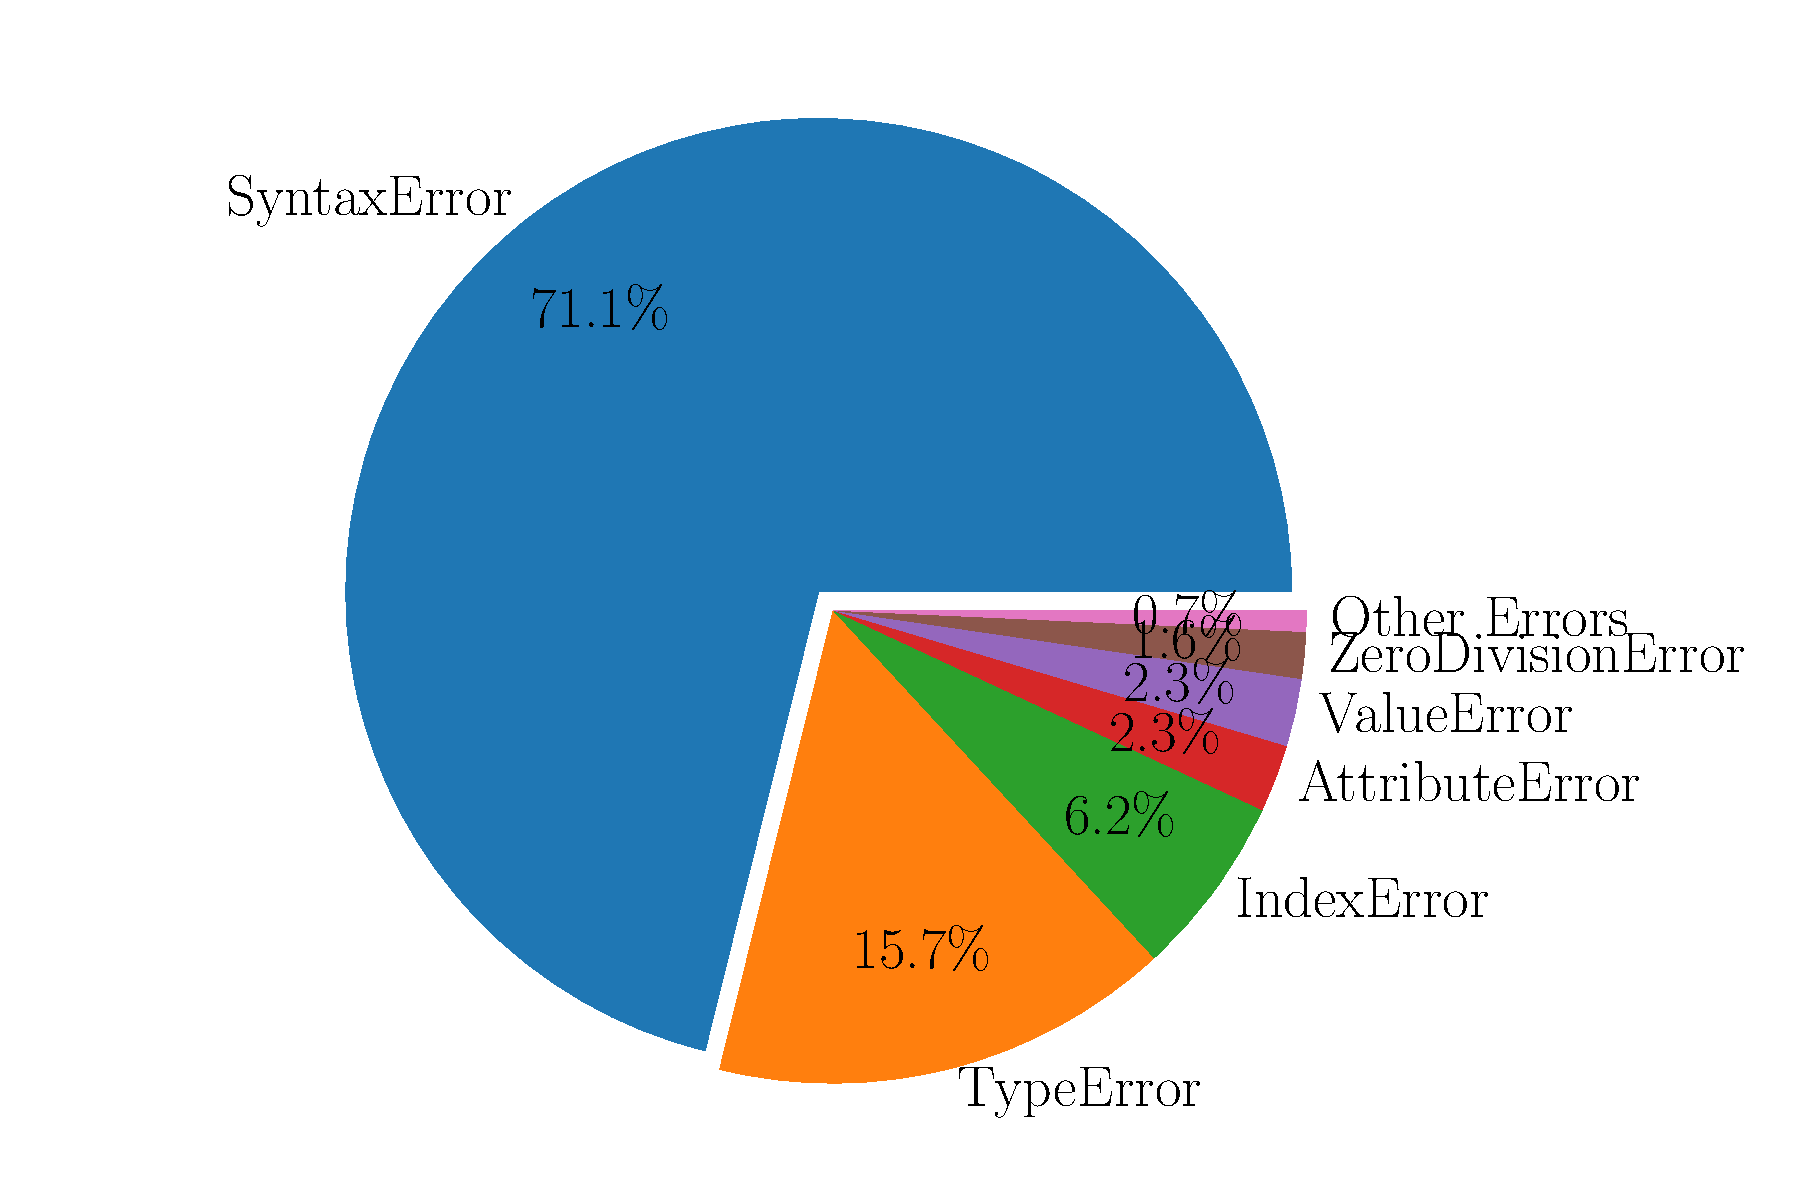
\includegraphics[width=\linewidth]{error-pie.pdf}
    \caption{The error type distribution.}
    \label{fig:error-statistics}
  \end{minipage}
  \begin{minipage}[c]{0.5\linewidth}
      \centering
      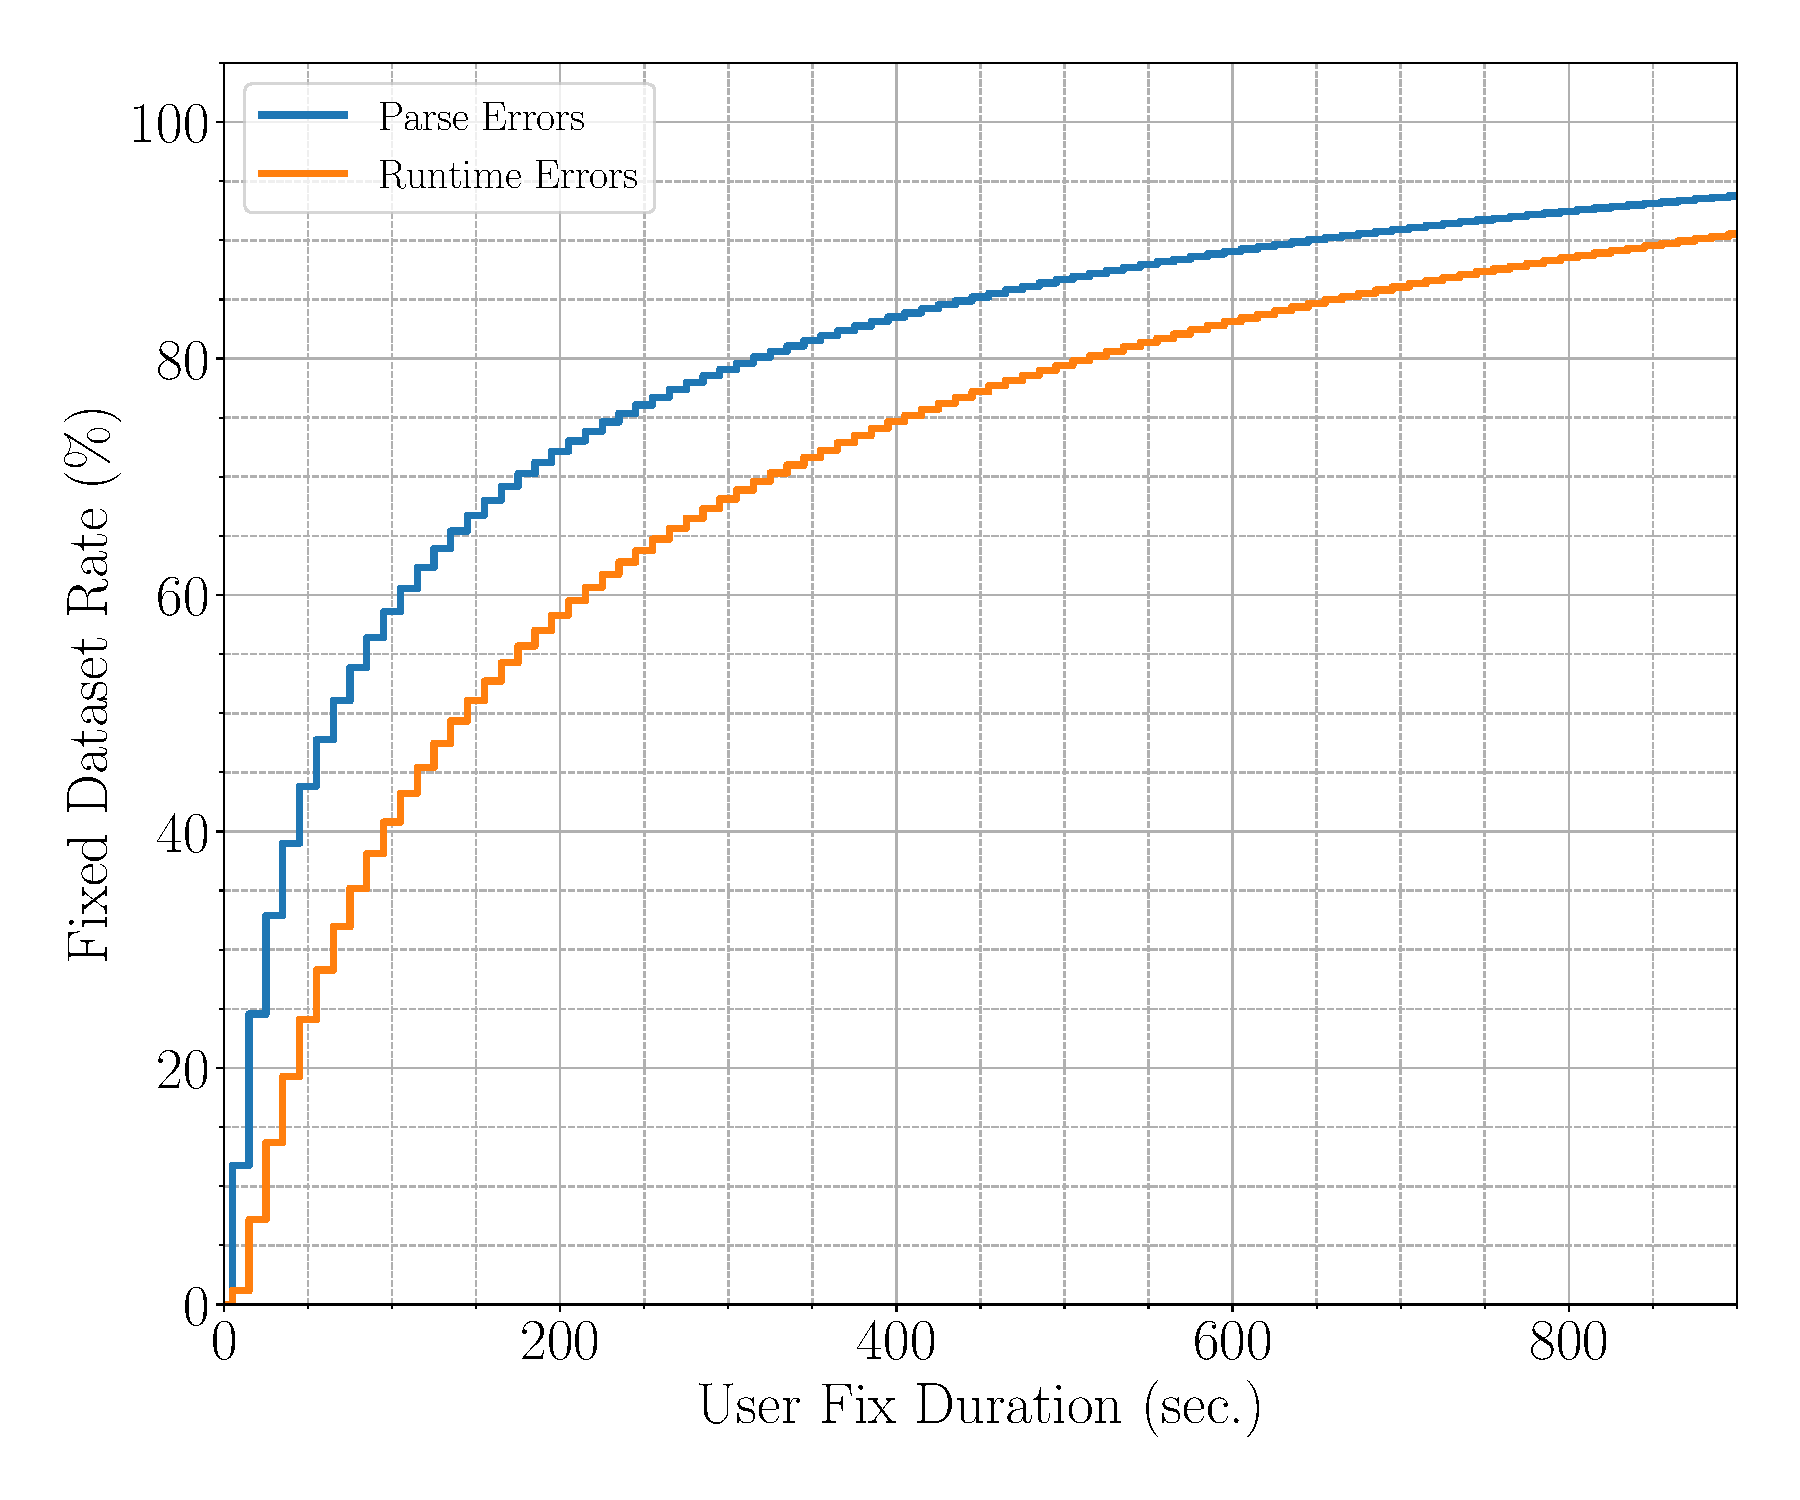
\includegraphics[width=\linewidth]{fixed-rate.pdf}
      \caption{The repair rate of the Python dataset for all, syntax and runtime
      errors.}
      \label{fig:repair-rate}
  \end{minipage}
\end{figure}

Parse errors (or \emph{Syntax Errors}) are usually easier to locate and be
repaired than other algorithmic or runtime errors most of the times
\citep{Denny_2012}. For example, the \emph{Python parser} will immediately
inform the programmer for missing parenthesis in function argument lists or for
not having the proper indents in a statement block. However, in this section we
show that programmers (especially novices) mostly deal with these kinds of
errors on a daily basis and spend a considerable amount of time fixing them.

\mypara{Python Syntax Errors}
We have collected a dataset of more than 1,000,000 erroneous Python programs
along with their fixes from a web-based Python compiler called
PythonTutor.com~\citep{Guo2013}, where novices programmers (mostly novices) can
submit their code online and execute it. When there is an error, the failed
attempt is recorded and associated with the next successful run of the same
fixed code. This process generates a dataset of program pairs.

By analyzing this data, we observe in \autoref{fig:error-statistics} that $77.4
\% $ of all faulty programs failed with a syntax error. This accounts for the
vast majority of the errors that (novice) programmers face with their programs.
This is a strong indication that these parse errors are very common and require
an automated approach of repairing.

\mypara{Python Repair Rate}
The web-based compiler that we used to generate our dataset, also provides us
with a \emph{server timestamp}. The timestamp is associated with each program
attempt submission, erroneous or not. The \emph{repair time} of an erroneous
program is calculated by taking the difference of the two timestamps of the
erroneous and fixed program. This method is not the most accurate, since there
are various reasons these timings are exaggerated, \eg users stepping away from
the computer, internet lag \etc. However, without loss of generality, due to the
large dataset of program repairs these timings can still be viewed as an
appropriate metric of the amount of time it took the programmer to repair the
errors in their program.

We plot in \autoref{fig:repair-rate} the \emph{programmer repair rate}, \ie the
dataset percentage that is repaired under a given amount of time. We include the
repair rate for all the errors, the parse/syntax errors and the rest of the
errors mentioned here as \emph{runtime} errors. As expected, the parse errors
are fixed faster than all the other ones, but not by a large difference. We
observe for example that within 2 minutes, usually $46\%$ of the runtime
errors, \ie all the errors that do not include the syntax errors, are repaired
and around $63\%$ of the syntax error. Although, this is a considerable
difference, we observe that there is still a large number of the "simpler" parse
errors that required more than 2 minutes to be fixed. We also observe that only
$48\%$ of the parse errors are fixed under 1 minute. Therefore, an automated
tool that repairs or parses those programs in a few seconds could be beneficial
for a lot of programmers, novices or not.

\begin{figure}[t]
  \centering
  \begin{minipage}[c]{0.49\linewidth}
    \centering
    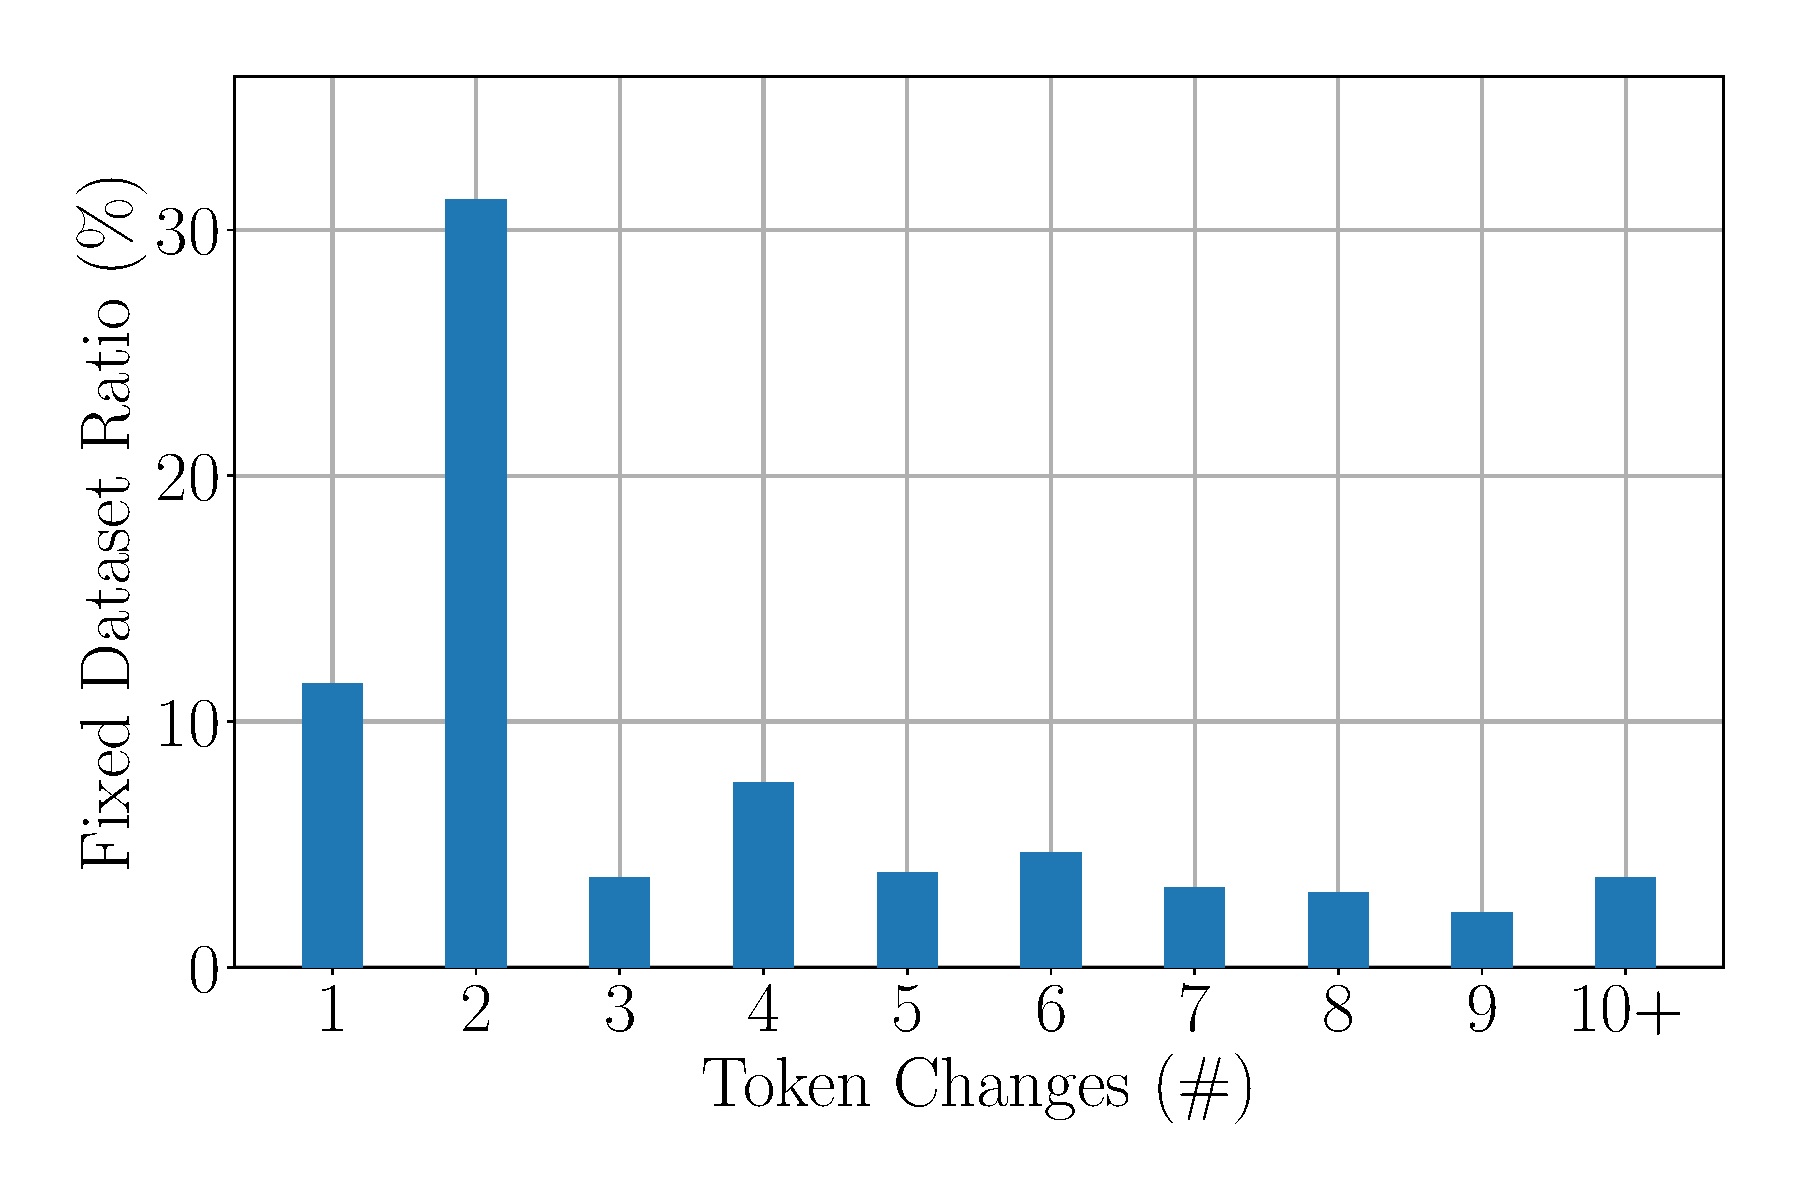
\includegraphics[width=\linewidth]{dataset-ratio-per-change.pdf}
    \caption{The Python dataset ratio that is fixed with the number of token
     changes needed to fix the erroneous program.}
    \label{fig:token-changes-ratio}
  \end{minipage}
  \begin{minipage}[c]{0.5\linewidth}
      \centering
      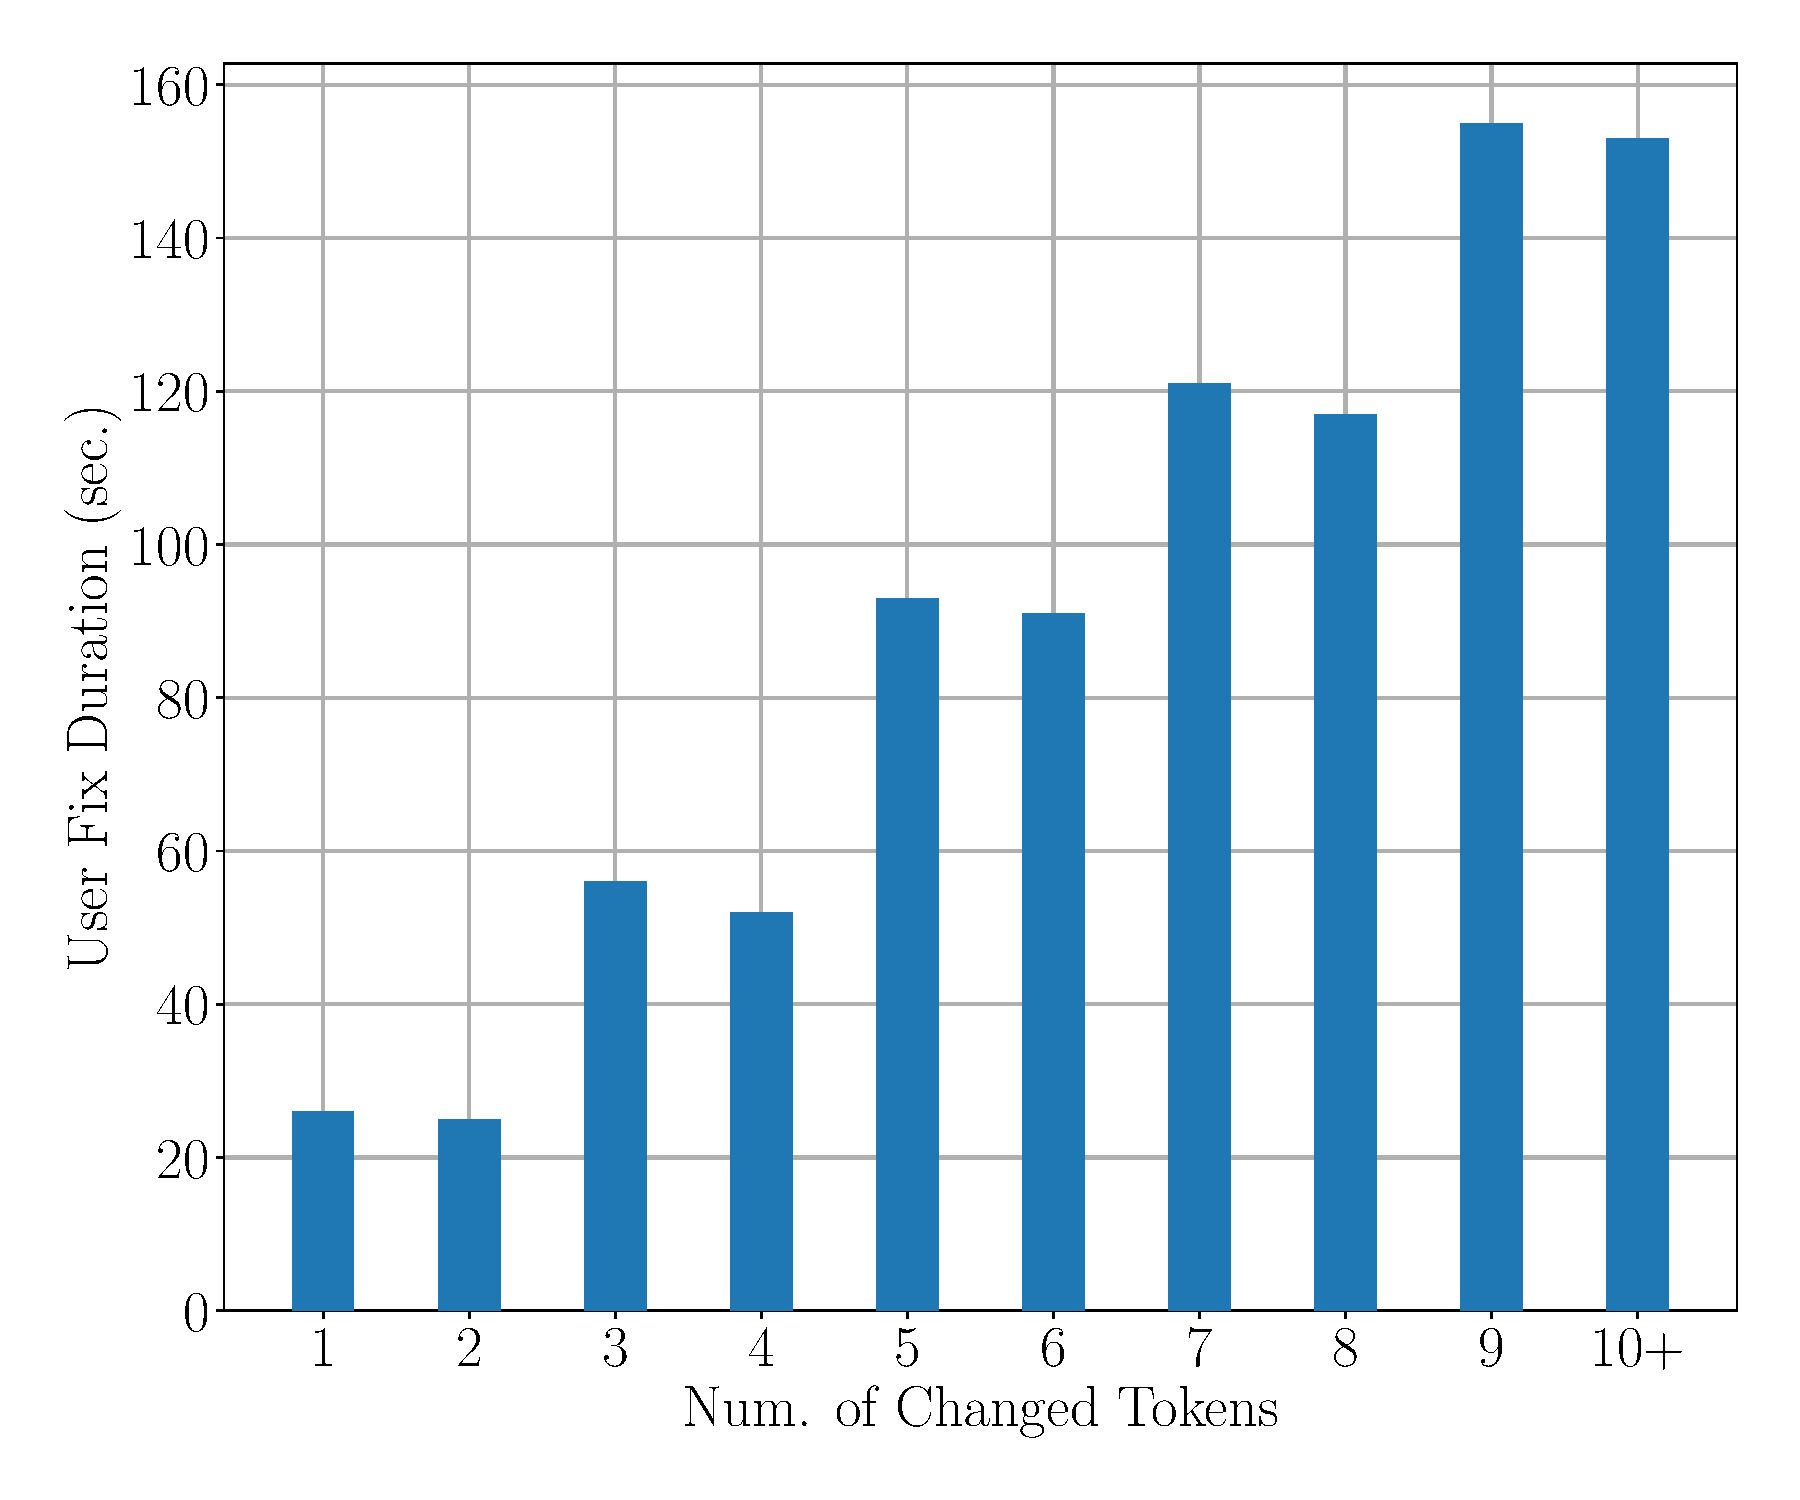
\includegraphics[width=\linewidth]{median-repair-times.pdf}
      \caption{The average time the user needed to fix the erroneous program
      under the number of token changes needed to make.}
      \label{fig:token-changes}
  \end{minipage}
\end{figure}

\mypara{Token-level changes}
The average token-level changes needed to fix a program with syntax errors, \ie
the number of changes in the lexed token sequence, is \emph{10.7 token changes},
while the \emph{median is 4}. A variable rename or a different integer is not
considered a change as they won't affect the syntax error fix. As shown in
\autoref{fig:token-changes-ratio}, $14.1\%$ of dataset needs only one token
change, $23.2\%$ needs two token changes, $7.0\%$ needs three and $9.0\%$ needs
four, \ie $53.3\%$ of the dataset needs at most 4 token changes to be fixed.
This shows that the majority of the syntax errors can be fixed with only a few
changes in their token sequences. But it is also important to see how long it
takes the users on average to make those changes.

\autoref{fig:token-changes} shows the average time that it takes a user to fix
their programs with syntax errors per the number of token-level changes in their
programs. As expected, with an increasing number of changes needed at program to
fix all parse errors, more time is needed for the programmers to make those
changes. Most importantly, even for one or two token changes the average user
spends 25.8 and 24.7 sec respectively, which is still a considerable amount of
time for these simple and short fixes.

These results further indicate that, while simple syntax errors can easily and
quickly be fixed by the programmers and the compiler error messages can be
helpful, programmers still struggle fixing programs that have more syntax
errors, that maybe the error message doesn't even point to.
